% file: 01-pattern-odd.tex

\documentclass[tikz]{standalone}
\usetikzlibrary{decorations.pathreplacing, positioning, arrows.meta, shapes.multipart, calc}

\begin{document}
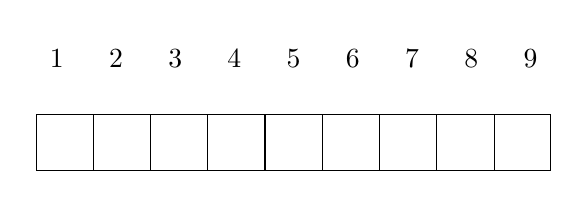
\begin{tikzpicture}[Array/.style = {rectangle split, rectangle split parts = #1, rectangle split horizontal,
    inner sep = 8pt, anchor = center}]
    % bit array
    \node[Array = {9}, draw] (A) 
    {\nodepart{two}\nodepart{three}\nodepart{four}\nodepart{five}\nodepart{six}\nodepart{seven}\nodepart{eight}\nodepart{nine}};

    % index
    \node[Array = {9}, above = 0.3cm of A] (A-index) 
      {1\nodepart{two}2\nodepart{three}3\nodepart{four}4\nodepart{five}5\nodepart{six}6\nodepart{seven}7\nodepart{eight}8\nodepart{nine}9};
\end{tikzpicture}
\end{document}
